\chapter{Cliques, Independent Sets and Vertex Covering }
Rishnak was eager to discuss other interesting problems with Ajur and  spotted Ajur and Jura walking along the shore of a pond. Rishnak asked Ajur about cliques in his school. Ajur readily shared his pet peeve with Rishank. Yes, students in his school belonged to distinct groups, essentially cliques. Then Rishnak told Ajur that a clique is also a graph theoretic term. A clique is a subgraph of a graph which is complete. Rishnak added that normally we only consider maximal complete subgraphs as cliques, that a maximal complete subgraph of $G$, $H$, means that there is no complete subgraph of $G$ that contains $H$ as a subgraph.

Rishnak drew the following graph in Figure \ref{13g1} and asked Ajur to list the cliques (maximal complete subgraphs).
\begin{figure}
\begin{center}
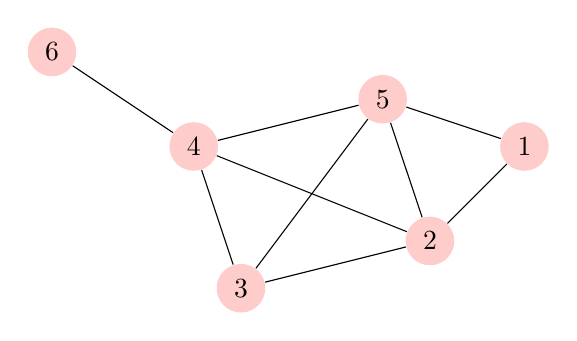
\begin{tikzpicture}
  [scale=.6,auto=left,every node/.style={circle,fill=red!20}]
  \node (n6) at (1,10) {6};
  \node (n4) at (4,8)  {4};
  \node (n5) at (8,9)  {5};
  \node (n1) at (11,8) {1};
  \node (n2) at (9,6)  {2};
  \node (n3) at (5,5)  {3};

  \foreach \from/\to in {n6/n4,n4/n5,n5/n1,n1/n2,n2/n5,n2/n3,n3/n4,n4/n2,n3/n5}
    \draw (\from) -- (\to);

\end{tikzpicture}
\caption{ What are the maximal cliques (complete subgraphs) in this graph}\label{13g1}
\end{center}
\end{figure}

Ajur was tentative in his answer - as he was struggling with all the definitions. He then stated that the three maximal cliques are: 
\begin{enumerate}
    \item Induced subgraph containing vertices 4 and 6.
    \item Induced subgraph containing the vertices 2,3 4 and 5
    \item Induced subgraph containing the vertices 1, 2 and 5
\end{enumerate} 

Rishnak was happy to note that Ajur understood the definition of maximal cliques. Still he wanted Ajur to find the
maximal cliques on another graph shown in Figure \ref{13g21}.
\begin{figure}
\begin{center}
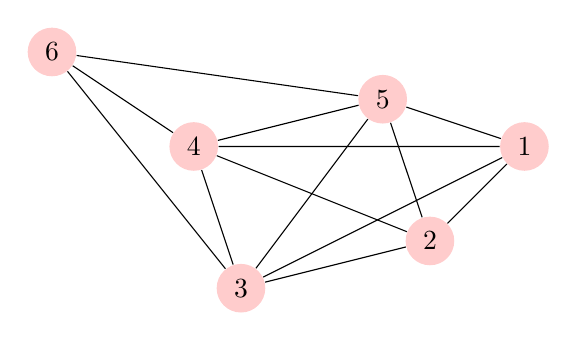
\begin{tikzpicture}
  [scale=.6,auto=left,every node/.style={circle,fill=red!20}]
  \node (n6) at (1,10) {6};
  \node (n4) at (4,8)  {4};
  \node (n5) at (8,9)  {5};
  \node (n1) at (11,8) {1};
  \node (n2) at (9,6)  {2};
  \node (n3) at (5,5)  {3};

  \foreach \from/\to in {n6/n4,n4/n5,n5/n1,n1/n2,n2/n5,n2/n3,n3/n4,n4/n2,n3/n5,n1/n4,n1/n3,n3/n6,n5/n6}
    \draw (\from) -- (\to);

\end{tikzpicture}
\caption{ What are the maximal cliques (complete subgraphs) in this graph}\label{13g21}
\end{center}
\end{figure}

Ajur stared at the figure \ref{13g21} for a few seconds, then answered, giving two maximal cliques. He listed them as: 
\begin{enumerate}
    \item Induced subgraph containing vertices 3, 4, 5 and 6.
    \item Induced subgraph containing the vertices 1, 2, 3, 4 and 5.
\end{enumerate} 
Seeing Ajur  frustrated with vague definitions and examples, Rishnak admitted that it was his mistake. Graphs are usually used as models for physical or social processes. For example, when we consider the cliques in a school, one can model the students as vertices and two students belong to the same group as an edge between the associated vertices\footnote{We have a binary relation here.}. Clusters in data science are closely related to cliques.

Rishnak then wanted Ajur to learn about Independent set in a graph. An independent set in a graph is a set of vertices that are mutually nonadjacent i.e., a subset of vertices that does not include any adjacent vertices. Ajur immediately recognized that Independent set and Clique are related. Rishnak could not control his smile. Rishnak remembered that he had not told Ajur about complement of a graph. A complement of a graph $G=(V,E)$ is another graph $H=(V,E_1)$. Both of them have the same vertex set. But if two vertices are adjacent in G, they are not adjacent in H and if two vertices are not adjacent in G, then they are adjacent in H. Ajur drew the complement of the graph (shown in Figure \ref{13g21})in Figure \ref{13g2}.

\begin{figure}
\begin{center}
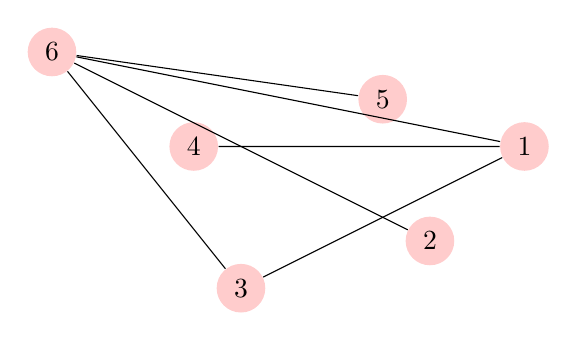
\begin{tikzpicture}
  [scale=.6,auto=left,every node/.style={circle,fill=red!20}]
  \node (n6) at (1,10) {6};
  \node (n4) at (4,8)  {4};
  \node (n5) at (8,9)  {5};
  \node (n1) at (11,8) {1};
  \node (n2) at (9,6)  {2};
  \node (n3) at (5,5)  {3};

  \foreach \from/\to in {n6/n5,n6/n3,n6/n2,n6/n1, n1/n3,n1/n4}
    \draw (\from) -- (\to);

\end{tikzpicture}
\caption{ Complement of Graph in \ref{13g21}}\label{13g2}
\end{center}
\end{figure}

Ajur further said that the number of edges in the complement of the graph will be $n\times\frac{n-1}{2}-e$ where original graph has $n$ 
vertices and $e$ edges. Hence a maximal clique in a graph will be an independent set in the 
complement of the graph. For the graph shown in Figure \ref{13g2}, the maximal independence sets are $\{2,3,4,5\}, \{1,2,5\}, \{4,6\}$ \footnote{Maximal here means that a super-set of it cannot be an independent set}. 
These are also the maximal cliques in Figure \ref{13g1}. In a bipartite graph shown below Figure \ref{13g3}, the maximal independent sets are $\{1,2\}, \{3,4,5,6\}, \{2,6\}$.

\begin{figure}
\begin{center}
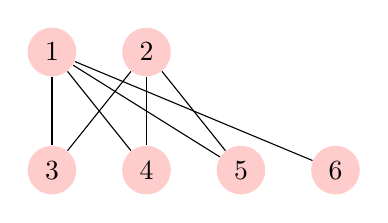
\begin{tikzpicture}
  [scale=.3,auto=left,every node/.style={circle,fill=red!20}]
  \node (n1) at (1,7) {1};
  \node (n2) at (5,7)  {2};
  \node (n3) at (1,2)  {3};
  \node (n4) at (5,2) {4};
  \node (n5) at (9,2)  {5};
   \node (n6) at (13,2) {6};
  
   \foreach \from/\to in {n1/n3,n1/n4,n1/n5,n2/n3,n2/n4,n2/n5,n1/n6}
    \draw (\from) -- (\to);
    \end{tikzpicture}
\caption{ A Bipartite Graph with 6 vertices and 7 edges}\label{13g3}
\end{center}
\end{figure}

Finding a maximal independent set is not hard, finding a maximum independent set is very hard - similar to finding a maximum clique. Maximum independent set refers to the maximal independent set which has the largest size. For the graph in Figure \ref{13g2}, the maximum independent set is $\{2,3,4,5\}$. For the graph in Figure \ref{13g3}, the maximum independent set is $\{3,4,5,6\}$.  Rishnak said that it is easy to find the maximum independent set in a tree. Ajur jumped up and down and said that he had a solution and described the following procedure. Ajur said that the input to his procedure is a rooted tree and the output is the maximum independent set.

Ajur also showed his procedure on the following example Figure \ref{13g4}.
\begin{enumerate}
    \item Let Maximum Independent set, $X=\emptyset$
    \item Add all the leaf vertices to a maximum independent set $X$.
    \item Delete all the leaf vertices.\footnote {Deletion of a vertex means delete a vertex and delete all the edges incident on that vertex}
    \item Delete all the newly created leaf vertices if there are any.
    \item Go to step 2, if the tree is not empty.
    \item $X$ is the maximum independent set of a tree.
\end{enumerate}

\begin{figure}
\begin{center}

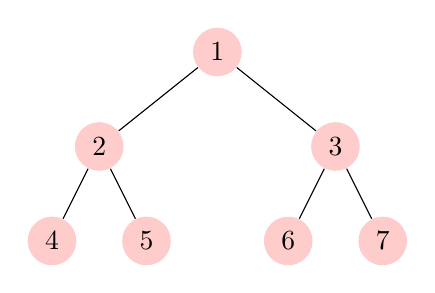
\begin{tikzpicture}
  [scale=.6,auto=left,every node/.style={circle,fill=red!20}]
  \node (n1) at (5.5,7) {1};
  \node (n2) at (3,5)  {2};
  \node (n3) at (8,5)  {3};
  \node (n4) at (2,3) {4};
  \node (n5) at (4,3)  {5};
  \node (n6) at (7,3)  {6};
  \node (n7) at (9,3)  {7};

  \foreach \from/\to in {n1/n2,n1/n3,n2/n4,n2/n5,n3/n6,n3/n7}
    \draw (\from) -- (\to);

\end{tikzpicture}
\caption{ The maximum independent set is $\{4,5,6,7,1\}$}\label{13g4}
\end{center}
\end{figure}

A closely related problem to Independent set is Vertex Cover. A vertex cover of a graph is a minimal subset of vertices that cover all the edges of a graph. Alternatively, if you delete all the elements in a vertex cover, the remaining graph will be an empty graph (that is, a graph with no edges). Intuitively, if we place policewomen in all the vertices of the vertex cover, then the policewomen will be able to watch all the edges (may be roads or corridors). Since we wanted to employ as few policewomen as possible, we want a minimal vertex cover.\footnote{minimal vertex cover means that no subset of it is also a vertex cover}
\begin{figure}
\begin{center}

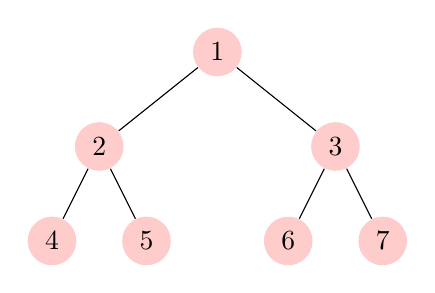
\begin{tikzpicture}
  [scale=.6,auto=left,every node/.style={circle,fill=red!20}]
  \node (n1) at (5.5,7) {1};
  \node (n2) at (3,5)  {2};
  \node (n3) at (8,5)  {3};
  \node (n4) at (2,3) {4};
  \node (n5) at (4,3)  {5};
  \node (n6) at (7,3)  {6};
  \node (n7) at (9,3)  {7};

  \foreach \from/\to in {n1/n2,n1/n3,n2/n4,n2/n5,n3/n6,n3/n7}
    \draw (\from) -- (\to);

\end{tikzpicture}
\caption{ The minimal vertex cover  is $\{2,3\}$ as all edges are incident on either 2 or 3}\label{13g5}
\end{center}
\end{figure}

Ajur said that vertex cover and independent set seem to be related. Rishnak smiled and replied if $X$ is a maximal independent set in a graph with $V$ as vertex set, then $V-X$ is a minimal vertex cover. Similarly if $Y$ is a maximum independent set and $V-Y$ is a minimum vertex cover. Ajur was impressed how all these seemingly unrelated sets are actually related. Ajur thought for a while and he said he understood how maximal independent set and minimal vertex cover are related. Maximal independent set, $X$, contains no edges as per definition. This implies that vertex set  $V-X$ covers all edges of the graph or every edge is incident in some vertex of $V-X$.

Rishnak wanted to test Ajur's understanding. He said that in olden days temples were constructed at the junctions of roads in a village. He asked Ajur, for the smallest number of temples that had to be constructed in the following Figure \ref{13g6} which shows the road map of Royt so that there is at least a temple at either end of each edge.
\begin{figure}
\begin{center}

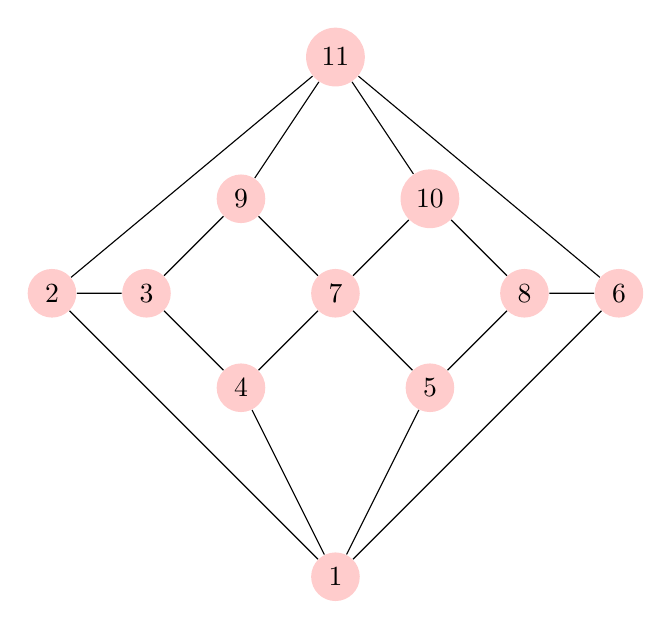
\begin{tikzpicture}
  [scale=.6,auto=left,every node/.style={circle,fill=red!20}]
  \node (n1) at (6,-3) {1};
  \node (n2) at (0,3)  {2};
  \node (n3) at (2,3)  {3};
  \node (n4) at (4,1) {4};
  \node (n5) at (8,1)  {5};
  \node (n6) at (12,3)  {6};
  \node (n7) at (6,3)  {7};
 \node (n8) at (10,3) {8};
  \node (n9) at (4,5)  {9};
  \node (n10) at (8,5)  {10};
  \node (n11) at (6,8)  {11}; 

  \foreach \from/\to in {n1/n2,n1/n4,n1/n5,n1/n6,n2/n3,n2/n11,n3/n4,n3/n9,n4/n7,n5/n7,n5/n8,n6/n8,n6/n11,n7/n9,n7/n10,n8/n10,n9/n11,n10/n11}
    \draw (\from) -- (\to);

\end{tikzpicture}
\caption{ Royt Village Road Map}\label{13g6}
\end{center}
\end{figure}

Ajur was mesmerized by the beautiful layout of Royt village. It looked so symmetric. He was tentative in his answer and he said that he would construct just 5 temples in vertices 11, 3, 7, 8 and 1.   When asked how he found so quickly. Ajur responded saying that he tried to find a minimum vertex cover for the Figure \ref{13g6} and he knew that would satisfy the temple requirements.

\textbf{Question for eleventh day} What is the size of the maximum independent set in a complete binary tree of height 5 (This will have 32 leaf vertices)

\textbf{Answer:} Ajur responded that the size of the maximum independent set will be 32+8+2 (vertices at alternate level) = 42 (as the minimum vertex cover size is 1+4+16=21).
Rishnak was impressed. It was getting dark and both of them called it a night.
